\documentclass{ubicomp2012}
\usepackage{times}
\usepackage{url}
\usepackage{graphics}
\usepackage{color}
\usepackage[pdftex]{hyperref}
\hypersetup{%
pdftitle={iPlant}, pdfauthor={Jesper Sandberg and Thomas Kokholm}, pdfkeywords={iPlant, Inteligent Plant System, Pervasive, Arduino}, bookmarksnumbered, pdfstartview={FitH}, colorlinks,
citecolor=black, filecolor=black, linkcolor=black, urlcolor=black,
breaklinks=true, }
\newcommand{\comment}[1]{}
\definecolor{Orange}{rgb}{1,0.5,0}
\newcommand{\todo}[1]{\textsf{\textbf{\textcolor{Orange}{[[#1]]}}}}

\pagenumbering{arabic}  % Arabic page numbers for submission.  Remove this line to eliminate page numbers for the camera ready copy

\begin{document}
% to make various LaTeX processors do the right thing with page size
\special{papersize=8.5in,11in}
\setlength{\paperheight}{11in}
\setlength{\paperwidth}{8.5in}
\setlength{\pdfpageheight}{\paperheight}
\setlength{\pdfpagewidth}{\paperwidth}

% use this command to override the default ACM copyright statement
% (e.g. for preprints). Remove for camera ready copy.
\toappear{Report written at the IT-University of Copenhagen for the course Pervasive Project Fall 2012. The copyright remains with the authors.}

\title{iPlant: Inteligent Plant System}
\subtitle{SPCL-2012 - Report Synopsis}
\numberofauthors{2}
\author{
  \alignauthor Jesper Sandberg\\
    \affaddr{IT University of Copenhagen}\\
    \affaddr{Rued Langgaardsvej Vej 7}\\
    \affaddr{DK-2300 Copenhagen S}\\
    \email{jesan@itu.dk}
 \alignauthor Thomas Kokholm\\
    \affaddr{IT University of Copenhagen}\\
    \affaddr{Rued Langgaardsvej Vej 7}\\
    \affaddr{DK-2300 Copenhagen S}\\
    \email{tkok@itu.dk}  }
\maketitle

\section{ABSTRACT}
People enjoy plants, their benefits and the feeling related to nurturing them. However for most people it becomes challenging to keep them healthy and alive. To accommodate this challenge we have developed a prototype, which makes a plant more self-sufficient, watering itself from a large water tank and providing itself with artificial sunlight.
The prototype reports status of its current conditions and also reminds the user to refill the water tank. The system automation is designed to be assistive to the user. We hope that through this prototype people will enjoy having plants without the challenges related to absent or forgetfulness.
iPlant is a step towards modern and future homes. Utilising the concepts of pervasive computing where users have complete control over their spaces \cite{future-homes}.

\section{AUTHOR KEYWORDS}
Plant monitoring, Automatic watering, Artificial sunlight, Wi-Fi Communication

\section{ACM CLASSIFICATION KEYWORDS}
Arduino, RHT03, Drip irrigation, Wi-Fi

\section{INTRODUCTION}

\hypertarget{introduction}
Since the dawn of time humans has lived with and enjoyed the beauty and benefits of household plants \cite{The-Benefits-of-Plants-and-Landscaping, houseplants-make-you-smarter} \cite[Chapter~2]{People-Plant-Relationship}. However since then, the way of nurturing plants almost haven't evolved. In a household plants are grown in mold or dirt, potted and placed on the windowsill. Due to this plants are dependent on regular nurturing - watering them and providing the right amount of sunlight to stay alive and grow. Plants are important for a healthy environment since they contribute to clean and natural air, with the production of oxygen \cite{photosyntese, light-for-plant-growth}. They help convert CO2 gasses and neutralize toxins in the air.

This has resulted in a number of challenges. \hyperlink{questionnaire}{Results of our survey} shows that people often forget to nurture their plant(s), between daily activities. \hyperlink{questionnairecomments}{The results we got from our survey} is that plants suffer and die, gets discarded and simply replaced by a new one, or \hyperlink{questionnaire}{as we discovered during the survey}, people stop having plants altogether. According to StatBank Denmark, Danes spend approximately DKK 2000,- per year on plants. This issue have even gotten as far as creating a successful industry for artificial/non-living plants made out of plastic.
People often develop a strong affection towards their plants, as we confirmed during our \hyperlink{questionnairecomments}{survey}). A relationship build on regular caretaking in order to grow and evolve - similar to the way animals and humans grow and evolve in life \cite{People-Plant-Relationship}. Research has shown that there is a link between nurturing plants as children, and how those children treat nature as an adult \cite{Childrens-Active-and-Passive-Interactions-with-Plants}.

In order to solve all or at least many of the above issues, engineers try to create helpful systems that keep plants alive by i.e. automatic watering or reminders like the Moreland AWS-10 \cite{moreland} or Botanicalls \cite{botanicalls}. However these systems do not solve the overall challenges. Plants still need humans as caretakers - one way or the other. So how can we solve all these issues, with forgetful humans, plants that require water and sunlight, as well as keeping the relationship between plant and people? Based on the above context, we believe there is a need for a home gardening system, which take care of all the different aspects in nurturing plants. We believe that technology can assist people in nurturing plants, not only by automation but also through digital communication (e.g. notifying a users when a plants is in needs of attention).

In this paper we explain how our system works as well as how it solves the above issues, we back up our theory of this system, by completing test scenarios on how well the system is able to perform in both a tough environment as well as a test in a real scenario environment. Based on the description of our system, our qualitative and quantitative research combined with our test scenarios we have drawn conclusions in order to show what we have achieved \todo{add more once we have finished the conclusion}. Overall we hope that this research will contribute to more people having the benefits of plants, as well as contributing to the advancement for design in homes of the future, e.g. home automation.

Furthermore we expect our prototype and research to show that automation doesn't necessarily remove or destroy the psychological aspects of care-taking plants. iPlant is intended to be helpful, assistive and smart.

\todo{add a small paragraph about your research method and process of the project to the end of the introduction}

\section{RELATED WORK}
\hypertarget{relatedwork}
In our work we focus on modern care-taking of plants and household gardening systems. The results of our survey show, that people do neglect care-taking of plants, from time to time. More than 70\% of the people in our survey mistakenly have killed their plants. Naturally different plants have different needs - not only in terms of attention, but also their environment. A paper by Mária Pohronská \& Tibor Krajčovič \cite{Handheld-Decision-Support-System} relate to this problem in their design of an embedded system for agriculture and home hardening. They use sensors to collect enviromental measurings, combined with knowledge base data, in order to recommend appropriate plants to grow on that location.

Make-Digital magazine posted a guide on microcontroller-assisted gardening \cite{how-to-make-a-gardening-system}, using an Arduino microprocessor, fluorescent light, a submersible water pump and 1" galvanized nails.

\begin{figure}[h!]
\centering
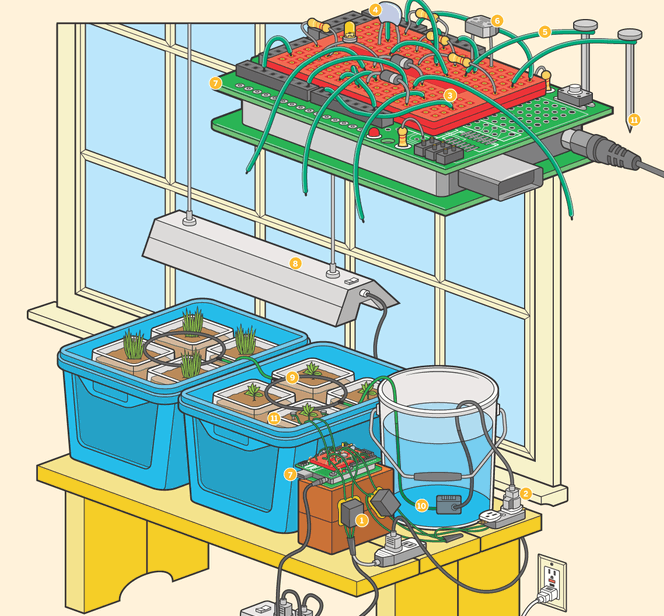
\includegraphics[width=\columnwidth]{howto-gardening.png}
\caption{Illustrating the scale and complexness of a do-it-yourself guide on microcontroller-assisted gardening \cite{how-to-make-a-gardening-system}. Image: Make-Digital Magazine.}
\label{fig:MakeDigitalMagazine}
\end{figure}

This system relates much to our idea, but the focus in the make digital guide is only on automation. Furthermore this gardening system is based heavily on a do-it-yourself concept. Our idea is just the opposite: designing a complete and finished solution, that is less demanding, and easy to use.

The scale of the MakeDigital solution is also very large, whereas our solution is small and compact. Even further, the Make-digital solution is highly complex to install, with lots of wiring and tubes going from bucket to bucket. See figure ~\ref{fig:MakeDigitalMagazine}

Most of the known commercial systems are based solely on having some sort of automatic watering, however the way these systems work are in most cases different.

For instance the Oasis Indoor Automatic Drop Watering System \cite{oasis-auto-drip} and the Moreland AWS-10 \cite{moreland} is simply a water-pump system based only on a timer, which can be programmed via an onboard LCD and buttons.

Easy2Grow Autopots \cite{autopots} on the other hand are based on gravity itself, where the water tank must be positioned higher than the rest of the system in order to work.

Systems like Moisture Matic \cite{moisture-matic} make use of a sponge wick to keep watering for up to 7 days.

CobroCo Plant Sitter \cite{plant-sitter} and the Self Watering Probes \cite{self-watering-probes} uses a ceramic sensor to measure when the plants need watering.

There are also systems like the Moisture Sensor Meter \cite{moisture-meter}, which only tells you the moisture level of your plant, but is not capable of watering.

The most interesting system in relation to our prototype is the Botanicalls \cite{botanicalls}, as this system is the only one to provide feedback based on user actions. It is similar to the Moisture Sensor Meter, in the way that it only measures the moisture, it is not able to water the plant, but it provides the extension of connecting to the Internet through a RJ45 Ethernet cable. By doing so it can provide features such as posting to your Twitter account when it is in need of water, also giving you a thanks when it gets watered.


In our research, we discovered that similar solutions that covers the same features as our prototype, requires large implementations and much wiring to setup. The solutions on the market today tend to take up a large amount of space. They relate more to greenhouse-installations than to regular household plants. Thus the target group often relate more to gardening enthusiast.

Our solution/implementation focus on household plants and is intended to replace regular pots, without being large- or bulky installations. The user's focus should remain on keeping plants - not on the technological or mechanical parts behind.

Our system will be assistive but not dominating. In contrast to other solution the user is still capable of watering the plant, without the system interfering.

Very few commercial gardening systems (intended for home usage) fully attend a plant’s needs. Most systems are based on watering only.

\begin{table*}[comparison_table]
\begin{center}
\renewcommand{\arraystretch}{1.5}
\begin{tabular}{| p{7cm} | p{3cm} |p{3cm}  | p{3cm} | p{3cm} |}
\hline
                                                    & Technology                        & Automation        & Interaction \\ \hline
        Moreland AWS-10 \cite{moreland}             & Timer                             & Water             & LCD \& Buttons \\ \hline
        Indoor / Outdoor Moisture Sensor Meter \cite{moisture-meter} & Sensor           & None              & Moisture Meter \\ \hline
        Easy2Grow Autopots \cite{autopots}          & Gravity                           & Water             & None \\ \hline
        Moisture Matic Automatic Watering System \cite{moisture-matic} & Sponge wick    & Water             & None \\ \hline
        CobraCo Plant Sitter Water System \cite{plant-sitter}   & Sensor                & Water             & None \\ \hline
        Oasis Indoor Automatic Drip Watering \cite{oasis-auto-drip} & Timer             & Water             & LED \& Selector \\ \hline
        Self Watering Probes \cite{self-watering-probes} & Sensor                       & Water             & None \\ \hline
        Botanicalls \cite{botanicalls}              & Sensor                            & None              & Twitter  \\ \hline
        iPlant                                      & Sensor                            & Water \& Sunlight & E-mail \& Web \\ \hline
\end{tabular}
\caption{Comparing the different features of various home gardening systems.}
\label{tab:Comparison-Table}
\end{center}
\end{table*}

In Table \ref{tab:Comparison-Table} we have compared 8 popular gardening systems with our solution.

We find that 4 out of 8 (excluding our own solution) are sensor based e.g. humidity. And all which is focused only on watering. None of them deal with sunlight. 
Furthermore only 2 of these systems have the ability to report status of the plant.

Except from Botanicalls none of the systems can communicate remotely to the user. Like most gardening systems, the user is forced to read the sensor values at the plant itself - which makes the readouts somewhat superfluous.

\section{BACKGROUND AND RESEARCH METHOD}

\subsection{Idea}
The main idea is to create a system that is capable of both watering and illuminate a plant. The system should be intelligent and capable of notifying the owner of the plants with status information obtained through sensors placed directly within a plant.

Furthermore users can combine multiple plants and monitor an entire villa through a web interface, or i.e. an office location with plants in different rooms, connected to a local Wi-Fi network. This ensures a natural work environment and provides all the information about the household plants accessible from the Internet.

Potting a plant combined with our solution provides a plant, with the necessary attention for it to sustain on its own for longer periods of time, even when located with no access to sunlight. Our solution will automatically water the plant regularly - keeping a fixed level of humidity in the soil.

Focus is on developing a prototype that is:
\begin{itemize}
    \item Small in scale
    \item Easy to use (and deploy)
    \item Ready from the beginning
\end{itemize}

iPlant should resemble regular household pots, yet packet with technology, assisting a user in nurturing household plants and provide users with information on temperature, humidity and general air. Using iPlant people can engage in having many different plants with absolute minimum effort. Even plants that require much attention like i.e. orchidaceae which are otherwise difficult to keep.

\subsection{Research Method}
\todo{should describe the process of your research: how you designed your system, how you identified the users’ requirements (questionnaire, interview, ...), and how you evaluate your prototype}

\subsubsection{Finding the Target Group}
Further research will have to be done in this area, but we decided to categorize our main target groups as the following:
\begin{itemize}
  \item Students
  \item Busy office/sales professionals 
  \item Families with several kids
\end{itemize}
With the most focus being on students.

\subsubsection{Questionnaire}
In preparing our questionnaire, we wanted to better understand and identify our respondents, as such we start our questionnaire with some demographical questions. Our next goal was twofold, to both identify the need and usability of our prototype, as well as making the respondents think about how common the issue we attempt to solve is. Our final goal of the questionnaire was to identify if our respondents believe our prototype to be the solution to this issue as well as describe any concerns they might have.

In conducting our questionnaire we decided to narrow down our respondents to our core target group, the students. This was done to get a more focused and deep (instead of broad) result of our questionnaire.
It should be put into consideration that most of our respondents are people we have reached through our Facebook, which could be people we know personally, this could affect the results in both a negative or positive way.

\subsubsection{Interview}
We have conducted two interviews with our volunteer for the human interaction test, Patrick. One at our initial meeting, where we explained the purpose of the test, how the system works and what we would like him to test during the test. We asked about his expectations and hopes for the system.
The final interview was conducted at the end of the test, we asked how it all went, what he thought of our prototype, any ideas, corrections, etc.

\subsection{Requirements Analysis}

\subsubsection{Fully Automated Scenario}
A family leaves their home for two weeks of much needed vacation. During their stay, their plants suffer from their absence.
In one room the curtains are closed, and prevent the plants from obtaining sufficient sunlight - they stop growing and begin to wither and may die.

\begin{figure}[h!]
\centering
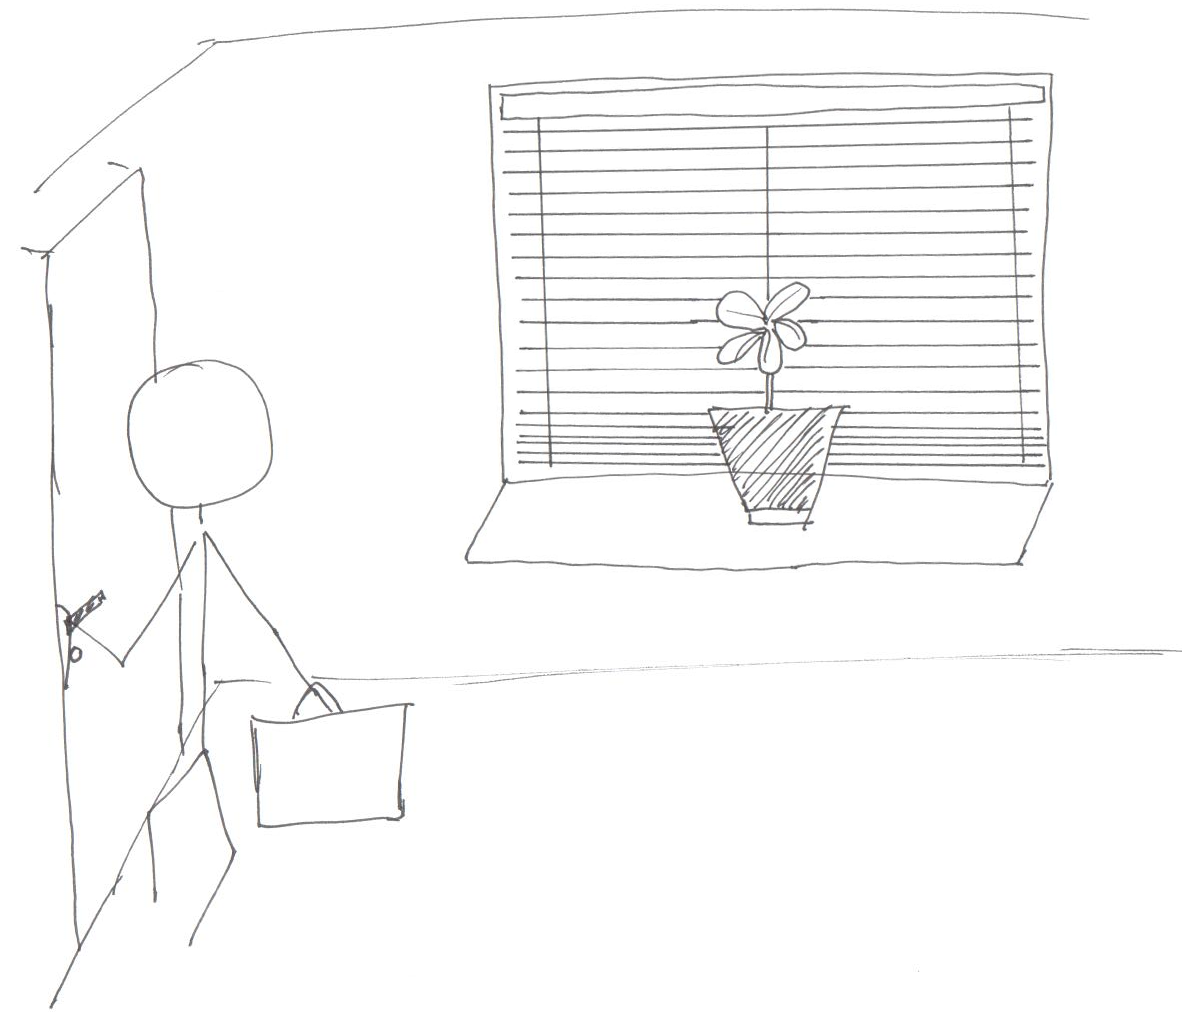
\includegraphics[width=\columnwidth]{closed_blinds.png}
\caption{Illustrating a scenario where closed blinds prevent the plant necessary sunlight.}
\label{fig:closed_blinds}
\end{figure}

In another room plants are over-watered in the hope that they will survive during the absence. They unfortunately drown from the massive watering.
In a third room the family did not water their plants sufficiently and wither from regular exposure to sunlight without moist soil to drain from.

\begin{figure}[h!]
\centering
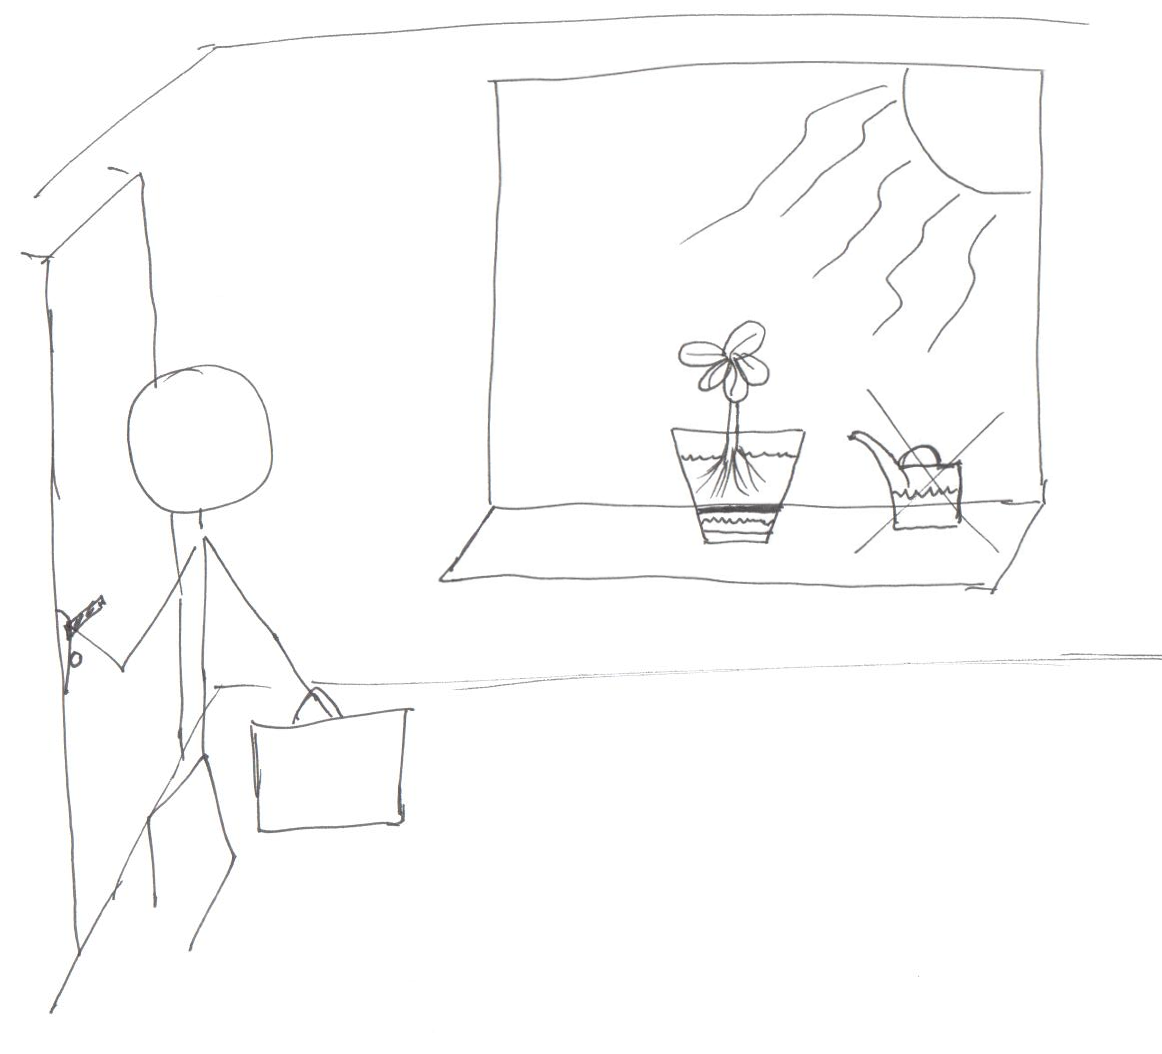
\includegraphics[width=\columnwidth]{forgot_to_water.png}
\caption{Illustrating a scenario where the owner neglects to water a plant.}
\label{fig:forgot_to_water}
\end{figure}

If only there was a system which could attend these plants, then the family would not only continue to have their plants upon return, they wouldn't ever have to worry when leaving home.

\subsubsection{Assistive System Scenario}
Bob love having plants in his house. He takes great interest in having many different plants. However Bob also has a very stressful job, that takes much of his attention. In busy weeks he sometimes forget to take care of his many plants. This has resulted in some of them dying and many getting close. Bob feels guilty about this and wishes there was something he could do to remember the plants in the weeks where he is so busy.

If there only was a system that could remind him or even help him when he forget to take care of a plant.

\subsubsection{Result of Questionnaire}
\hypertarget{questionnaire}
We got a total of 66 respondents of which 61 (92.4\%) completing the questionnaire. 83\% are students and 89\% are 20-29 years of age with a slight overweight  of male respondents.
Of this group 72\% have over-watered a plant, 94\% have forgotten to water a plant (see Figure \ref{fig:MakeDigitalMagazine}), 69\% have forgotten to pull up the blinds or curtains and 78\% have killed a plant.
56\% would consider paying money to get a system such as our prototype, the average maximum amount being DKK 238,- for the system.

\subsubsection{Result of Interviews}
For our initial interview we spent most of the time setting up the system and explaining how the system works, we asked for his expectations of the system, he simply replied that he did not know, but he guess he was expecting the plant not to die.

For the interview after the 2 week test we asked him what he thought about having the iPlant in his home, he mentioned that it was smart and very futuristic. As this was part of the human interaction test, we asked what he thought about the notifications, to that he said that he did not like the ones where the plant is simply reporting back that it is doing fine, he even compared it to spam and would like some function to disable them. We would like to know if a system like this would make him want to get more plants, to this he answered yes, but only if it was possible to disable those notifications. He also thought that this makes having plants less boring. In wrapping things up we asked if there is anything else he would like to have changed with the system, to this he mentioned that he got a little tired of refilling the water tank, because it was so small.


\section{SYSTEM ARCHITECTURE}
Based on the survey results our focus is on designing an intelligent plant, with inspiration drawn from similar systems such as Make Digital's guide to a home gardening system \cite{how-to-make-a-gardening-system} and Botanicalls \cite{botanicalls}.

iPlant is designed to be "smart" and assistive: helping a user attend household plants. It is focused on automatic watering and artificial sunlight, combined with sensors and Wi-Fi internet communication.

iPlant is a step towards modern and future homes: utilizing the concepts of pervasive computing, where users have complete control over their spaces. As envisioned by Stephen S. Intile \cite{future-homes}: 
\begin{quotation} \em...our homes will be so fully automated and “smart” that we will rarely have to think about everyday tasks at all.
\end{quotation}
With iPlant the user has the ability to nurture plants, and rely on the system to monitor the plants and act to sustain the plants health. Users can and will still be able to nurture plant on their own without the systems interfering. The system is designed to be assistive (e.g. watering the plant if the user forgets to do so). iPlant can even be set to feedback only, and simply inform a user of a plants status and health.

\subsection{Hardware}
\subsubsection{Wi-Fi Module}
iPlant communicate remotely through a Wi-Fi connection, established within a user’s private network. Wi-Fi connections are accessed using an Arduino Wi-Fi Shield \cite{arduino-wifi}.

Through the internet, iPlant can send messages to a user. Informing the user of sensor readouts, i.e. environment temperature, humidity or how many hours of sunlight the plant has been exposed to. Messages are currently emailed to the user, but could be any internet service i.e. a webpage, a twitter account etc.

All data regarding the plant is stored and logged for online monitoring. The user is always capable of remotely checking the current status of a plant. Furthermore the user can change threshold values for automatic watering and UV-diodes and including all the settings regarding notifications (e-mails), or schedule time intervals for automatic nurturing (e.g. when on vacation).

\subsubsection{Central Processing Unit}
iPlant handles all digital input/output and analog signals, using an Arduino Uno microprocessor board, based on the Atmel ATmega328 \cite{atmel328,arduino-uno}. It is a low power CPU (Central Processing Unit), ideal for simple calculations. It is extremely reliable, embedded computer. Conveniently small to fit our prototype gardening solution.

\subsubsection{Submersive Waterpump}
Using a modified submersive water pump from Moreland gardening \cite{moreland}, iPlant is capable of pumping water from a container and thereby watering the plant. The water pump is connected to the microprocessor, which signals the pump to turn on and off.

\subsubsection{UV-diodes}
The system illuminates a plant using UV-B LED diodes \cite{uv-diodes}. The diodes provide artificial sunlight as an energy source for the plant \cite{fotosyntese}.
%UV-diode with 410nm wavelength

\subsubsection{Lightdetection Sensors}
In order to detect sunlight on the plant, iPlant uses light detection sensors \cite{light-sensors}. 

\subsubsection{Galvanized nails}
iPlant uses 1 inch galvanized nails buried in the soil in order to know the humidity of the mold. The resistance between the nail compared to the input voltage gives an indication of the humidity - enough to detect if the plant has been watered or not.

\subsubsection{Humidity \& Temperature Sensors}
iPlant is equipped with a humidity and temperature sensor component. Checking the environment temperature and humidity of where the plant i located. Too high or too low temperature and humidity reading can be bad for certain plants. The user can verify the environment from a web interface or get notified by the gardening system by e-mail.

\subsection{Software}
\todo{Here goes everything about the web interface, user settings, notifications (messages) etc.}
The user is capable of viewing all the collected data on our user web interface (see figure \ref{fig:web_overview}). Here the user can read all the sensor values manually and through periods of time from all the loggings iPlant have collected. 

\begin{figure}[h!]
\centering
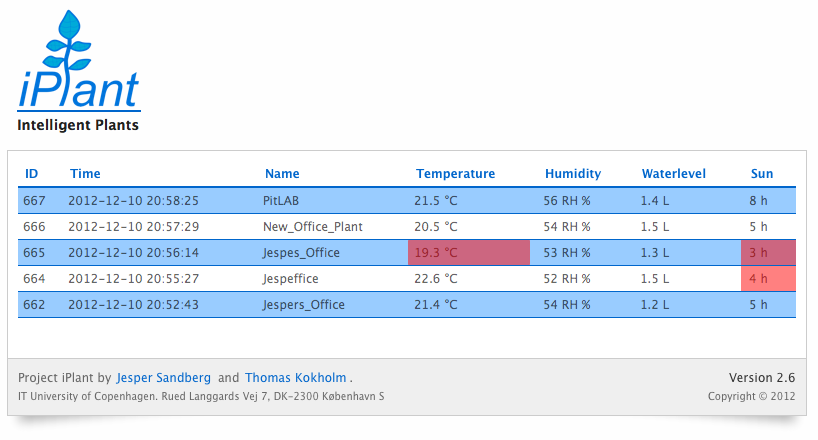
\includegraphics[width=\columnwidth]{web_overview.png}
\caption{Screenshot of iplant.dk web user interface. Red markings highlights if a sensor value is below its threshold.}
\label{fig:web_overview}
\end{figure}

The user can also change all the settings of a plant. Changing the threshold values of e.g. minimum humidity, water and temperature. Also communication settings like WiFi name and password can be changed remotely.

\begin{figure}[h!]
\centering
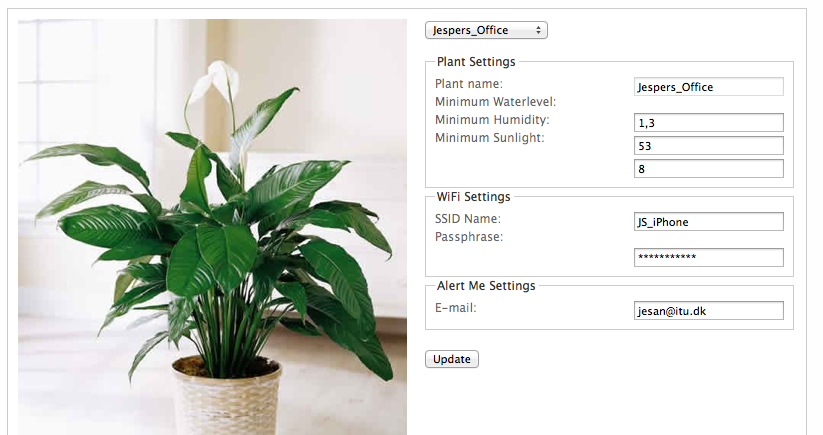
\includegraphics[width=\columnwidth]{web_settings.png}
\caption{Screenshot of iplant.dk web settings interface. Thresholds define the minimum accepted state of water level, humidity, temperature and sunlight. Also showing notifications and communication settings.}
\label{fig:web_settings}
\end{figure}

Furthermore the user can define which email the notification should be addressed to (See figure \ref{fig:web_settings}).

Notifications are email messages sent from our iplant.dk server. They are automatically generated with messages based on the collected sensor data and thresholds assigned by the user on the web interface. The emails is written like the plant is talking to the owner.
An example notification could be: 
\begin{quotation}
\emph{Hi [username]
Today I feel fine, the sun is shining on me and I have plenty of water :-) }
\end{quotation}
or if the plant suffers:
\begin{quotation}
\emph{Hi [username]
You forgot to open the blinds for me, I don't like to be in the dark. But I will survive on UV light. Please remember me :-( }
\end{quotation}

\subsection{Design}
%Include our design process, iterations, prototypes, design decisions, drawings, video, etc.
Our first design iteration was drawn upon a piece of paper[reference or figure], on which we both illustrated scenarios and tried to figure out how the prototype should be designed, eg box-type or bucket-type. We ended up deciding that the best result would be to have a prototype that looked as close as possible to the average household potted plant.
Our second design iteration was a video prototype, in which we showcased and explained our idea and several scenarios.
\begin{figure}[h!]
\centering
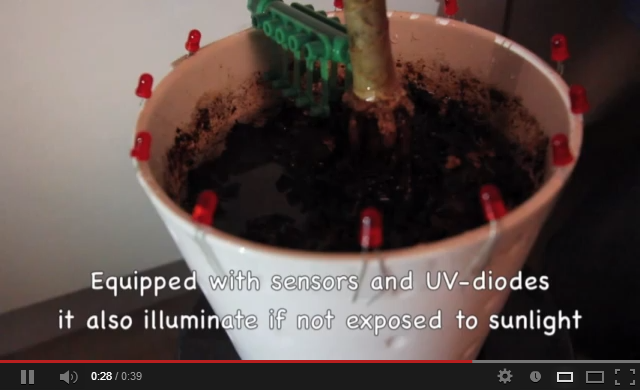
\includegraphics[width=\columnwidth]{iPlant_youtube.png}
\caption{Screenshot of our video prototype on YouTube. (http://www.youtube.com/watch?v=lk3Jyxf1szc)}
\label{fig:iPlant_youtube}
\end{figure}
During the development and testing of the mentioned hardware above, we have developed several prototypes, in which we have tested each component separately before putting it all together to the final prototype.

\todo{Add figure and references}

\subsection{Relation Aspect}
For an introduction to this section, please see section \hyperlink{introduction}{INTRODUCTION}, which explains the mentioned issues.

In order to try to compensate for some of these issues, we have developed a feedback feature to our plant management system, note that this feedback is customizable, so that users can receive e-mails from the plant, telling them about how they are doing. These messages will not simply be hard data and facts, but be structured in such a way so that the plant is speaking like a normal person would and even joking about its condition and what is currently going on in its life.
We do this to not only enhance the joy of having a plant, but to keep and further develop the relationship between plant and owner. This is done by the continuously communication back and forth, with the owner watering the plant and the plant expressing its joy and thanks to the owner, which in turn should make the owner more engaged and happy with his plant.

The iPlant system will have the ability to entirely disable automatic parts, so that only the monitoring part maintain active. This will ensure maximum satisfaction for all users.

\section{EVALUATION \& RESULTS}
For our evaluation we use a combination of qualitative, quantitative and longitudinal \cite{longitudinal} research.
The qualitative research will be done as interviews in relation to our human interaction test as described below, we combine this with our quantitative research, which is done as questionnaires in order to get data from many people, which we can rely on and use to draw conclusions as well as discover challenges with our prototype. The longitudinal research is carried out for our human interaction test, as our prototype consists of a plant, which takes a considerable amount of time for changes to happen. The combination of these three research methods will give us a reasonable background and data to draw reliable conclusions regarding our plant management system.

\subsection{Test Settings}
The test i performed in a fixed indoor environment, eliminating wind, fluctuating temperatures and irregular sunlight, as a source of error. 
Our test subjects is two equally identical plants, both from the same family, and they are given the same amount of mold and water to begin with.

\subsubsection{Stress Test}
In order to test the survivability of our prototype, we arranged a stress test. In the test we potted a plant in our iPlant solution and compare it with a regular potted plant. 
The testbed setup is located underground, in a basement. The basement is completely dark with no windows. Temperatures in the basement scale with the outdoor temperature, but is around 10 degrees celsius warmer. We set up the plants and leave them for a period of 3 weeks.

\todo{Finish the test and add pictures}

\subsubsection{Human Interaction Test}

In order to see and understand how humans interact with our prototype, we have arranged a human interaction test. A real scenario, as close as possible to how we expect the final solution.

In this test, we try to understand some of the relationship aspects that exists between humans and their household plants \cite{People-Plant-Relationship}, and see if and how our prototype affects these relationships.

With focus on human interaction we arranged an longitudinal test with Patrick Andersson (27) male from Copenhagen, living in a small apartment volunteered to try our prototype for 2 weeks.

The test was involved Patrick nurturing the plant as if it was a regular potted plant. He received notifications based on email messages from the plant (through our server) informing him about the plant’s health. It also notified him when or if the plant had been assisted (e.g. watered or given sunlight).
%Write about our human interaction test, which is testing our system in a real scenario in a home with humans not related to the project - nurturing the iPlant.
%Explain the different challenges and results of this test, focus on the human aspect. How the plant is perceived, refer to interview(s) with the humans from our test scenario.
%Answer:
%+ Can it work? and if not why?
%+ Does it become more boring to have plants?

%simulte the finished beutiful system. Where would people place the plants. What problem arise and etc.
\subsection{Interview}
Patricks first impression of the system is that it is 100\% self reliable, that he dosent have to do anything, and that the plant will still survive no matter what. While this would be great, the user still has to attend to the system from time to time. Refilling the water tank, and making sure that the plant dosent get any diseases. Power outages or other outside factors could disable the current prototype completly without notifing the owner.

Patrick thought the system was very futuristic, that confirms our assumption that our prototype will fit younger people well in accordence to adapting new technology.

Patrick found some of the notifications redundant and annoying. We proposed an alternative solution where the notifications could be filtered, for instance only notifiying if something is wrong and avoiding messages like "everything is fine".

Patrick reported that he would like to have more plants in his house if they were all based on the iPlant system. As having only one self sufficient plant is obsolete, as he would still need to attend all the remaining plants.
Patrick would like the water tank to contain more water, so for future prototypes we would make the tank larger, so the plant could survive even longer.

Patrick believes having plant systems like this makes life easier and better, however we don't think that everyone shares his believe, especially not plant enthusiasts.
%Hvad har du af forventninger til systemet?
%Det ved jeg ikke. Forventer vel at planten den ikke dør.

%Hvad syntes du generelt om at have iPlant i huset.
%Det var smart! Meget futuristic.

%Hvad syntes du om notifikationerne?
%Ingen spam tak, en funtion hvor man kan slå emails fra. Sådan ikke at iPlant ikke hele tiden mailer om at alt er godt.

%Ville du have flere planter i lejligheden med dette system?
%Han vil gerne have flere planter, hvis det da var fordi han havde sådan et system til dem alle sammen.

%Er der noget du synes skulle ændres ved systemet?
%Træt af at skulle vande beholderen. Beholderen var for lille og skulle alt for tit fyldes op.

%Synes du det er blevet mere kedeligt at have planter med et system som iPlant?
%Nej det er meget bedre!

\subsection{Questionnaire}
As most of our respondents are young students, there is a low tendecy in purchasing plants, especially more expensive plants, however still more than half of the respondents indicated that they were willing to purchase our prototype.

Almost everyone of our respondents have at some point forgotten to water their plants. Most respondents reported that they had also forgotten to pull up blinds and over-watered their plants. Only every 5th respondent said that they had not experienced killing a plant.

The primary group of our respondents are young people under the age of 30, which fits our solution very well, since young people is often faster and better in adapting new technology. They are also most likely the owners of future smart homes, which could include our system.

\begin{figure}[h!]
\centering
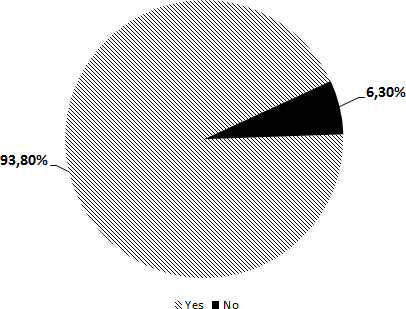
\includegraphics[width=\columnwidth]{diagram_forgotten.jpg}
\caption{Procentage of respondents that have forgotten to water their plant.}
\label{fig:Questionnaire}
\end{figure}

\hypertarget{questionnairecomments}
Respondent at 28-11-2012 11:11 PM:
\begin{quotation}
\em I don't care that much about plants. When it dies (like it always does at my house) I'll just buy a new one.
\end{quotation}

A big part of our prototype is exactly to take care of this problem, instead of spending money on buying new plants all the time, you can simply get one that will not die.

Respondent at 28-11-2012 8:57 PM:
\begin{quotation}
\em Having plants is not ment to be automatic for me. The reward for a plant to "bloom" will give less satisfaction than if your did it by hand. - I see the that it would be smart for holidays ...
\end{quotation}

Our system also works for this situation, in which you can disable the automatic part and only use the notifications, in case you forget to water the plant. For holidays you can simply re-activate the automatic part of the system.

Respondent at 5-11-2012 5:09 PM:
\begin{quotation}
\em I enjoy caring for my plants. I would not be interested in a device which did that for me, but I WOULD however, be very interested in a device which could help me optimize my care taking. For example, if it could give me plant-specific feedback about water, light, and soil (more - less etc.) I would like that very much. In essence, it would help me learn what each particular plant likes best.
\end{quotation}

This is exactly the idea of our notification system, which will assist you by sending you e-mails when you need to water the plant, when plant have not received enough sunlight, etc.

\section{DISCUSSION}
\todo{Discuss the challenges of our system, with high regard to our evaluation and results. Also discuss and evaluate the future use, work and applications for iPlant.}

\todo{Pros og cons}

\todo{Future work}
%Discussion: være kritisk

During the 3 weeks of stress testing our solution, we noticed how the leaves turned and folded downwards towards the diodes. The leaves tend to arrange themselves towards the light. In a future version we would address this issue be rearrange the location of the diodes to hang above the plant lighting downwards on the plant instead.

\section{CONCLUSION}
\todo{Draw conclusions from what is written in the above sections.}

\nocite{Smart-Homes-and-the-People-Who-Live-in-Them}
\section{ACKNOWLEDGEMENTS}
First and foremost we would like to give our thanks to our teachers Thomas Olof Pederson \& Shahram Jalaliniya.

A big thanks to Sebastian B\"uttrich and the ITU pITLab for guidance, tools and materials.

We would like to give our thanks to the assistance of Amager Planteland.

Thanks is also given to our volunteer Patrick Andersson.

\vfill\eject

\bibliographystyle{abbrv}
\bibliography{sample}

\todo{Make appendix with questionnaire diagrams, comments, etc.}

\end{document}
